%
% $Id: ch03_thework.tex
%
%   *******************************************************************
%   * SEE THE MAIN FILE "AllegThesis.tex" FOR MORE INFORMATION.       *
%   *******************************************************************
%
\chapter{Method of Approach} \label{ch:method}
In order to create an effective image matching algorithm, it was necessary to pull research, knowledge, and pre-existing code from a number of resources in addition to completing original code. Although the research does not target the hardware infrastructure of the network that image sharing sites use, a simple public web server was built and configured. This topic will be briefly discussed in Section \ref{sec:serverconfig} To test the proposed image matching method, it was also necessary to build a skeleton that would act as a simple image sharing website. This skeleton is capable of accepting an image file and returning a link to the user which will allow the submission to be viewed. The site also allows for the development of the proposed matching function and will provide the necessary functions to accept and handle the output of the research.

\section{Server Configuration} \label{sec:serverconfig}
In order to implement the website, it is necessary to have an environment capable of running the required processes. To do this, several options were considered. The first option was to run the site on a locally installed Apache web server. After a small amount of testing, this was determined not to be the best option. Due to the lack of a dedicated machine the web server had wildly varying performance due to interference from other processes that could not be closed. This was even a problem when operating with a fixed amount of memory. In addition to this, the XAMPP environment was also tested for performance. This environment gets its name from the functionality it provides pre-configured and out of the box. In other words, X (Cross-Platform) Atache HTTP Server with MySQL, PHP, and Perl. This package functions across any operating system platform as a fully functional web server. In many cases the configuration is acceptable as is, but in the case of this research, even after changing resource limits and other settings the software still frequently became non-responsive with resource hungry processes such as analysis of large files.

The next alternative was to purchase web space on a shared server. These servers are readily available at minimal cost from dozens of providers such as A Small Orange, BlueHost, and Byethost. After careful consideration several concerns prevented the use of this method. The primary factor was that these servers are shared with numerous users. Due to the nature of this setup, it is unknown how many websites are being hosted by a particular server, and how many concurrent users are accessing these sites at any given time. In addition, it is not possible to set an allotted amount of memory for a particular environment or control what programs are running that may possibly impact the performance of the research.

Another option that looked very promising at first was to rent server time from a provider such as Amazon Web Services. With this method not only it is possible to control what programs are operational, but it also allows for more freedom of configuration. This would seem like the most promising solution to the problem, but there are still factors that cannot be eliminated, such as the speed of the Internet connection at any given moment. By hosting a local web server, it is possible to control this factor, but the issue remains of how much it could affect the results. To test this concern, a server was rented using the free tier of services. From this point, a simple timer was configured and one 15 megabyte file was transferred using SFTP. This process was repeated 10 times and the results were analyzed. After reviewing the results, there was no concerning transfer speed variance, making this a good match. In the end, it was discovered that there are restrictions on the service that do not allow an individual to alter server settings relating to resource allocation, which was a key concern from the start.

The final option was to implement a local dedicated web server and operate the website and scripts from that. The machine allows not only very tight control over variables such as resource allocation, installed programs, and custom network hardware configuration, but it also allows usage on a local network or over an internet connection. By running initial tests on a local area network, it is possible to eliminate Internet speed fluctuations and control the number of devices utilizing the network bandwidth. This also opens another path where a real world simulation can be run by submitting images to the system over an internet connection and comparing the behavior with only one variable at a time differing.

To build the server a specification had to be determined that would allow optimal performance. To allow the greatest flexibility, the Ubuntu Server operating system was chosen. From this, the server's hardware specifications were chosen based on the minimum system requirements given by the operating system, Apache suite, and MySQL Database. This information was used to pick a quantity of memory, hard disk space, and processor speed. The server was built with 4 gigabytes of random access memory (RAM), 3 gigabytes allocated to the programs and operating system, a 2.43 GHz Intel Core i3 processor, and dual 7200 RPM 500 gigabyte hard drives. The integrated network card was faster than the available network equipment, so it was not of direct concern. The hard disks were chosen to provide ample space for any reasonable number of tests but not provide so much space as to be considered excessive for their purpose. A 7200 RPM variant was also chosen to allow the maximum data throughput and not become a bottleneck when working with great numbers of large image files. Finally, the disks were configured as a redundant mirror to emulate a simple backup system that duplicates the data as a form of backup. This allows the collection of data and comparison of storage requirement improvements in a non-redundant system, and one with a worst case scenario backup implementation that simply creates copies of the files.

The software selection is more straightforward. After selecting to use a Linux operating system, Ubuntu Server was chosen as the distribution. I had the most experience with using, configuring, and troubleshooting issues with this environment and decided it was best for this reason. The accompanying software was fairly simple to select as a quick Google search for ``Ubuntu web server'' will return thousands of results outlining the setup and configuration of a basic Linux-Apache-MySQL-PHP, or LAMP server. The setup process was completed step by step using the ApacheMySQLPHP LAMP Server Setup Guide provided through the Ubuntu Documentation \cite{ubuntu:lampsetup}. Next, the code which will be discussed shortly requires that the PHP GD Image Library be installed. To prepare the PHP installation to use this library, the server was configured using the direction of the tutorial hosted by nixCraft \cite{nix:gdsetup}.

Upon the completion of the prior configurations, the server was updated and running the latest version of all installed software. To prevent updates from altering the outcomes of the future, a hold was placed on all packages to prevent all non system security related updates from being installed. In addition to this, the firewall was configured to allow HTTP communication through port 80, which allows interaction through an internet browser with the website hosted on the server. This was followed by a reconfiguration of the connected network router giving access to the internet through port 80. MySQL did not require any setup past the installation of the program and was left alone. At this point, the server configuration was complete and the default Apache ``Success'' page was displayed when accessing the server showing that everything was working properly.

\section{Website Design} \label{sec:websitedesign}
The core of this research hinges on the successful implementation of an image comparison algorithm. In order to do this, a website needed to be developed that acted in a manner similar to a simple image sharing site. In order to do this, a specific demographic of users had been targeted. Due to the code limitations of the PHP GD Duplicate Image Finder written by CatPa \cite{catpa:gdcode}, only jpeg submissions are accepted for the purpose of this research. In addition to this, a 15 MB file size limit is enforced. This is to prevent excessive wait times when transferring the image file to the server during tests run on a large number of files. The website was designed to be lightweight; more specifically, it has no extraneous scripts or applets running on the upload page. The purpose of this is to give processing times relating only to the actual upload process and not nonessential scripts. Finally, the last restriction placed on the website development is cross browser compatibility. Instead of placing focus on making a website that functions across all common web browsers, it was decided it would be highly beneficial to work with the Gecko browser platform, such as Firefox, due to the vast array of development tools available. This limitation will also allow for a focused effort in file management on a specific platform and will allow room for further research after the tool has been optimized.

To begin, a database was implemented in such a way that it holds a vast array of information. The image sharing functionality of the website requires several different pieces of information to be stored in a database. The first column of the database houses the identifier for each entry. This is known as the primary key, which is a column in a database where all entries must be unique and the key is used to identify the information in the row. This identifier is used by the website to track the order of the submissions to the server since the date uploaded is not important to the research and will not be tracked. The next column, as seen in Figure \ref{fig:schema}, is the {\tt ILookup} column. This is what the website uses to look up each image location on the server when supplied with a URL containing this identification code. This column must always have a value so the {\tt NOT NULL} flag was set. The third column is {\tt IName}, the column that houses the actual file name of the image being stored on the server. This column must also have a value so the {\tt NOT NULL} flag was set. This is concatenated to the end of the {\tt directory} entry which cannot be null, and provides the website with the exact location of the image file on the server with respect to the Linux root directory.

Each of the remaining database columns are specific to the image de-duplication scripts. First, the {\tt uMethod} column is nothing other than a single integer that marks what upload method was used to place the image on the server. If this number is set to ``0'', the image was uploaded using the non-duplicate reducing functions. On the other hand, if this number is set to ``1'' it is known that the image was uploaded and checked for duplicates before committing to long term storage. Both the {\tt hash} and {\tt fingerprint} fields contain information that allows the scripts to rapidly search the database for duplicate files when a new file is uploaded.  Both of these columns are allowed to have a null value. This is allowable due to the fact that non duplicate reduced images will not have any image matching data associated with them. These non duplicate reduced images will be discussed in Section \ref{ch:reseval} when discussing the base case that the results will be compared to. Finally, the last column tracks the total time in milliseconds that it took to upload the image to the server. This is not allowed to be null as both the base case and the duplicate reduced case will require this information. In Section \ref{ch:reseval}, this data will be used to compare the resulting data gathered by uploading images in a traditional manner and using this duplicate reduced function being researched.

\begin{figure}[htbp]
\centering
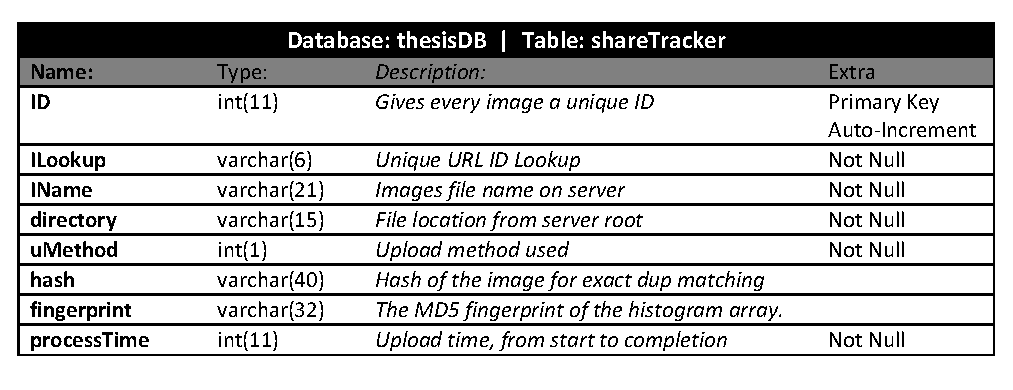
\includegraphics[width=6in]{schema}
\caption{Schema for file uploads.}
\label{fig:schema}
\end{figure}

In order to test the effectiveness of the research being discussed, a base case must be created against which to compare the results of running the algorithms. To create this data, the website performs one function before moving on to the duplicate reduction test. A separate directory was created on the server where every single image submission will be placed regardless of whether it is duplicate or not. This will mimic the upload process of a non-duplicate reducing image sharing website. Each entry into this folder will be placed in the database exactly the same as the duplicate reduced entries are, but will contain no image identification information. This first process is referenced henceforth as a traditional upload method. This upload method is unknown to the user as it will not return a URL allowing access to the image at a later time. During this process, each file is assigned a new, unique name to prevent collisions upon upload. A SQL {\tt "INSERT"} will then be run on the database for the image and will record the file's location on the server, the file name, the fact it was uploaded using the traditional method, the unique URL to access it from (which is not given to the user), and an {\tt ID} for each insert into the database. After the completion of the process an {\tt "UPDATE"} will be run on the database entry created by the {\tt "INSERT"} above. The time taken to complete the task will then be included in that entry and can be used to analyze the efficiency of both systems upon the completion of the tests outlined in Section \ref{ch:reseval}.

After the initial upload completes, a second script is called. The second script has been designed to operate in two steps. This function performs mostly the same tasks as the traditional upload, but checks the image being uploaded for duplicates and handles each case appropriately. First, the image will be matched in the most basic form by hashing the image file using an MD5 file hashing function, after which the resulting hash will be compared to all images in the database using the following SQL Statement: {\tt "SELECT * FROM `share\_tracker' WHERE `uMethod' = `1' AND `hash' = `fileHash'"}. If this statement returns any results relating to a matching hash on a duplicate reduced uploaded image, it has found an exact matching image. 

In the event where a match is not found, the script will continue to the second stage of duplicate finding function. This function will operate in several different stages. The first stage toward finding an approximate image match is creating a fingerprint of the image file. In order to do this, the script will create a GD image object by using the PHP GD Image Library that was configured on the server in Section \ref{sec:serverconfig}. After the object is created, the GD Library has built in functions that allow iteration through every pixel in the image and view each pixel's red, green, blue value, or RGB value. These values will then be used to return a fingerprint in the form of an MD5 hash of the color frequency of the image. This color frequency is also known as a color profile. The next step to identifying a duplicate image would be to query the database for any images that have a perfectly matching color profile. This profile will be the same for an image no matter the variation as long as the image resolution, color and contrast are left unmodified. At this point, if there is no matching color profile, it can be said that there is most likely not a matching image on the server and
the function will return no matches found.

If the color profile does in fact match that of one or more images on the server, the script will then make a $16\times16$ pixel full color copy of the image being uploaded in addition to $16\times16$ copies of each of the images with a matching color profile. This process will also utilize functions provided by the GD Library that will allow pixel by pixel comparison of each image. When re-sizing an image, a number of techniques can be used when changing the total number of pixels. One popular method of re-sizing an image is called interpolation. With this process, when reducing the number of pixels, the algorithm will select one pixel and any immediate neighbors to it, at most there will be four. The algorithm will take the values of all five pixels and average them together eliminating the need for the neighbors as the original now represents the values of all five.

This process is continued pixel by pixel until the image has reached its desired smaller dimension \cite{Acharya:2007}. This fact will allow the comparison of both images even if they were different dimensions, as the resulting $16\times16$ files will have similar averages after re-sizing if they are in fact a match. Because of a possibility of slight variations in color, this function will not look for exact match, but will allow a set amount of deviation between two thumbnails.

To compare the pixels of both images, the RGB values of the corresponding pixels on each image will be analyzed. First, the red value of a pixel will be subtracted from the red value of the corresponding pixel's red value in the other thumbnail. The absolute value of the difference will be recorded. The same process will be completed for the green and blue values of that pixel. Once the difference from that pixel is calculated, the same comparison will be performed on each of the remaining pixels. In order to allow for very slight variations in color with each pixel, the resulting total calculated deviation will be divided by the number of pixels to `normalize' the result. After that calculation is complete, if the final deviation is less than or equal to the limit set by the website administrator, the function will return that a matching image was found.

If after all of the above processes are completed and no duplicate image is located on the server, the image upload will be accepted by the function and stored on the server's disk. At this time a SQL {\tt "INSERT"} will then be run on the database for the image and will record the file's long term location on the server, the file name, the fact that it was uploaded using the duplicate-reduced method, the unique URL to access it from, the image's MD5 hashed histogram that is described below, the thumbnail created for histogram comparison, and an {\tt ID} for each insert into the database. After the completion of the process an {\tt "UPDATE"} will be run on the database entry created by the {\tt "INSERT"} above. A view of the functioning duplicate-reduced upload process can be seen in Figure \ref{success_nodupfound} when no duplicate image is located.

\begin{figure}[htbp]
\centering
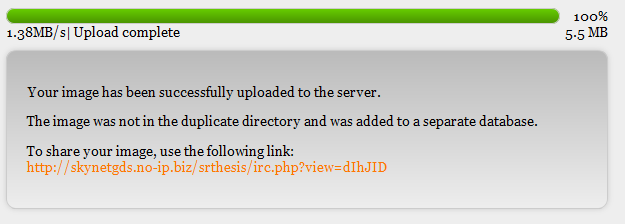
\includegraphics[width=5.5in]{success_nodupfound}
\caption{Successful image upload response when no duplicate is located.}
\label{success_nodupfound}
\end{figure}

If the image is determined to be a match after the completion of the full image hash function or the completion of the color profile and $16\times16$ pixel by pixel comparison, the submitted image is assumed to be a duplicate and a prompt will be displayed to the user showing the image they provided and the possible match that already exists. If the image is verified a match, the user will be given a unique link to the image that is already on the server, and the image being uploaded will be discarded as a duplicate. At this time the system will run an {\tt "INSERT"} on the database linking the new identifier to the image already on the server, and it will be added to the database. If the user decides the image is not a duplicate, the system will run an {\tt "INSERT"} statement and it will be added to the database. Following the completion of this process an {\tt "UPDATE"} will be run on the last {\tt "INSERT"} and the time taken to complete the task will be included in that entry. A view of the functioning duplicate-reduced upload process can be seen in Figure \ref{success_dupfound} when a duplicate image is located.

\begin{figure}[htbp]
\centering
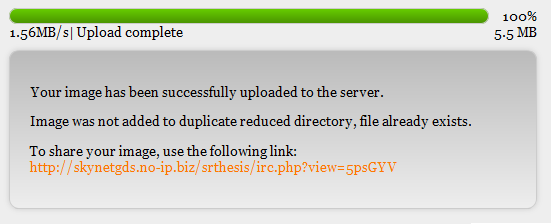
\includegraphics[width=5.5in]{success_dupfound}
\caption{Successful image upload response when a duplicate is located.}
\label{success_dupfound}
\end{figure}

In the case of requiring duplicate files, where the user decides to upload the image regardless of uniqueness, the script will be able to differentiate between the two images with the unique image ID that is generated at the time of insertion into the database. The closest matching occurrence of an image on the server compared to a new upload will be used in the prompt and displayed to the user. This will prevent frustration with multiple prompts every time more than one duplicate is found. This technique will also allow multiple links that point to the same image while leaving the user unaware of the system operating in the background to provide a consistent experience. An outline of this full process can be seen in Figure \ref{method-fig1}.

\begin{figure}[htbp]
\centering
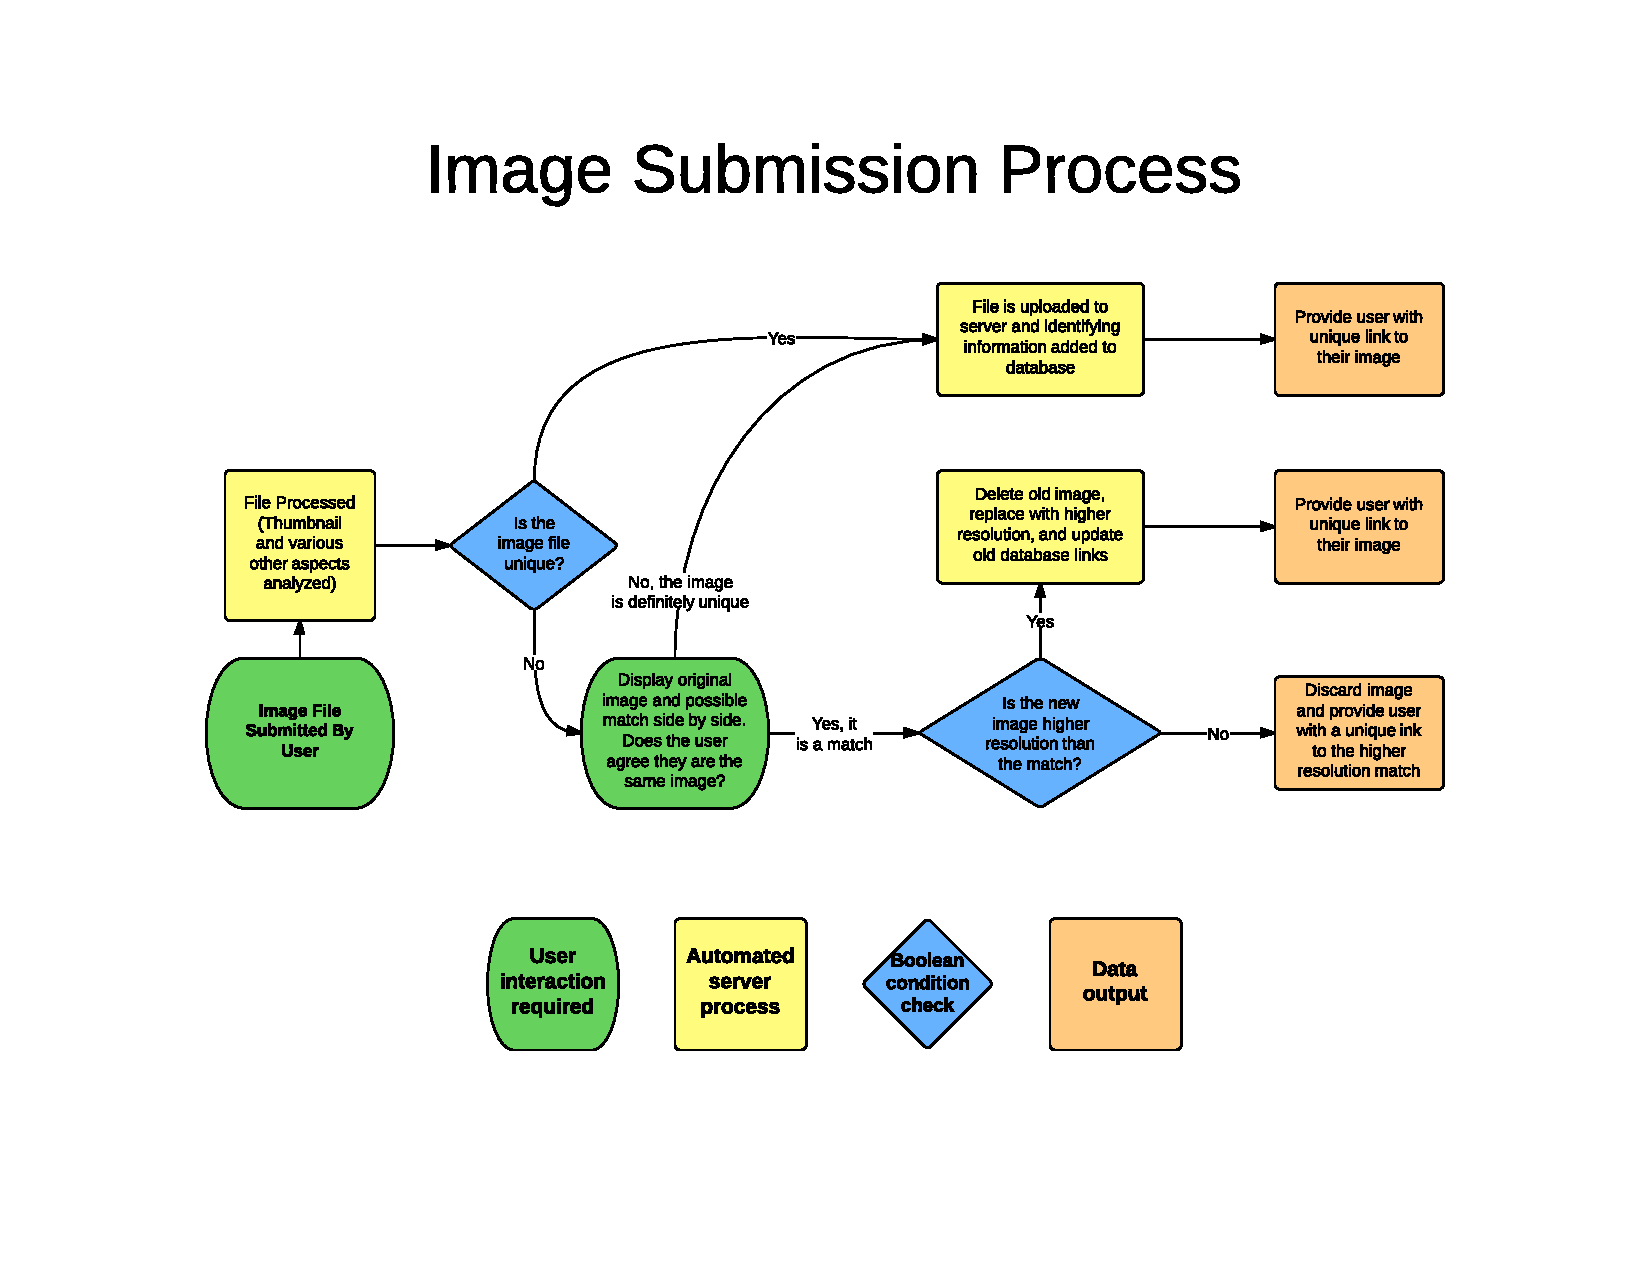
\includegraphics[trim={3cm 3.5cm 2cm 4.2cm},clip, width=6in]{upproc}
\caption{Streamlined upload process.}
\label{method-fig1}
\end{figure}

When a user accesses the file from the provided link, the system will run a query that looks up the image identifier provided in the URL. If it matches an image on the server, the image location will be used to provide the image to the user for viewing. The user never notices a difference, but on the server side we have ensured file redundancy has been eliminated and possibly improved user experience by providing the user with higher quality content than what they were expecting. If the requested image is not found, a 404 ``Image cannot be found'' error will be displayed to let the user know something went wrong.

\section{Color Profile and Histogram Comparison} \label{sec:histogram}
As mentioned in Section \ref{sec:websitedesign}, an image is composed of RGB values associated with every pixel in an image. In order to use these values in an effective manner, a thumbprint of the color profile had to be created. This color profile is represented as a histogram and allows the visualization of each color's frequency. This section will break down the process of comparing histograms and their accompanying data and explain the reasoning behind the comparison method chosen for this research.

As mentioned before, each pixel in an image is composed of an RGB value that allows the storage of the correct mixture of each color in that pixel. This value is separated into three separate ranges of 0-255 values where the higher the number the brighter the color. As seen in Figure \ref{historep}, a histogram has been generated using a popular photo editor by the name of Paint.NET. On the right hand side the four different overlaid histograms can be seen. The `x'-axis represents the relative number of occurrences of each 0-255 value while the `y'-axis represents the values themselves. The red layer indicates the frequency of each red value, the lowest of the 0-255 values being at the bottom of the image, and the highest at the top. The green and blue indicate the same for their respective colors. Also, note that blacks, whites, and grays can be represented by the RGB values. For example $255,255,255$ represents a solid white pixel while $000,000,000$ represents a pure black pixel, thus these colors do not require their own array.

\begin{figure}[htbp]
\centering
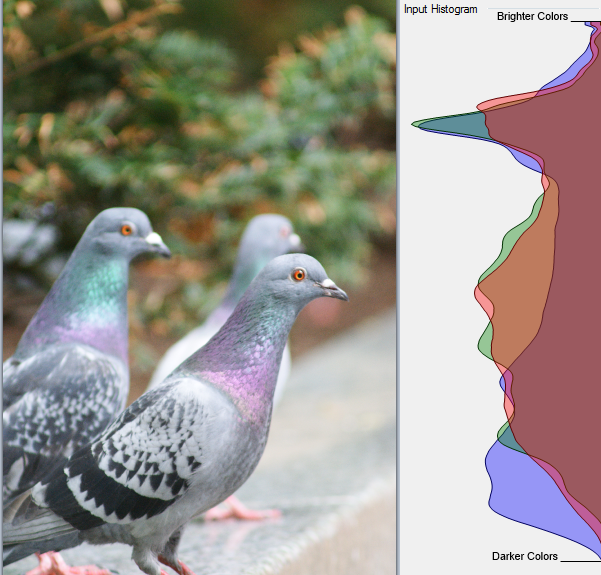
\includegraphics[width=4in]{historep}
\caption{Visual representation of an image's histogram.}
\label{historep}
\end{figure}

This collection of values that make up the histogram is where the comparison process begins. For any comparison of data to occur, each pixel's RGB values must be recorded into three arrays of size 256. The index of the red, green, and blue arrays will correlate to the 256 possible colors within the respective color. As a color is encountered, a counter in the code will increment the value by one at that array index. This will allow the tracking of the frequency of each of the RGB values. It does not matter what pixel these are related to as the overall number and frequency of each color is the only concern.

At this point, every RGB value in the image should be stored within the color's respective array. This is the array of values that can be graphed using a histogram, and the visual of the color profile can be printed out for visual inspection. Since we will be using a function to process the values, the actual generation of said histogram would be unnecessary. These values can be handled and compared in a few ways, but the best method for the purpose of this research much be chosen. This array could be processed using the PHP {\tt serialize()} function and stored in the database for later examination. By doing this, each of the arrays would require separate serialization, and all three would require their own columns. With this method, the array could be pulled from the database and run through the {\tt deserialize()} function to return the array to its original state. This would be beneficial for applications that would require the comparison of each individual array index to another array. Due to the large amount of processing time required to iterate over multiple arrays of size 256, this is not optimal. In addition to this, we are not concerned with calculating the difference in color profiles, but are only concerned with an exact match. The use of exact-only matching is valuable with this research topic. If two images with different color profiles are being compared, it will be assumed that they are distinct. An identical color profile could potentially signify a duplicate image as explained below.

The color profile requirement better lends itself to a different method of histogram value comparison. Due to the fact that we need to find only exact matches and that the system accounts for a possible false positive, hashing the three arrays will suffice. For this process, the three arrays will be concatenated in the order {\tt Red.Green.Blue}. This will generate one array with 1020 indexes representing the separate counts of each individual R, G, or B color value. This value will then be taken and processed with the PHP $md5()$ function which will return a 40 character alphanumeric string representing the array. When an uploads fingerprint is created, the database will be searched for an exact match hash. If a matching hash is found, it is known that a photo with the same color profile is already on the server. In the event of a hash collision where two different histograms have the same resulting hash, the script will be performing a pixel by pixel comparison anyway and will be able to decide that the images are not unique, so this is not of concern.

Due to the fact that the only images of concern are exact color profile matches, it is not required to store the values of the color profile in a recoverable format. This leads away from storing either a plain text array of values in a database, or storing a serialized version of the array in the database. Because of this, it is acceptable for a 40 character alphanumeric hash to be stored in the database and directly compared to the hash of a newly submitted image in order to detect a possible duplicate image.

\section{Threats to Validity}  \label{sec:threats}
With any area of research comes inherent shortcomings no matter the care taken to eliminate free variables. By creating a locally hosted server and excluding any extraneous scripts from the website, these variables were controlled to the greatest extent possible. Due to the nature of a publicly hosted web server, there is always a chance of malicious attack which could skew the results one way or another. As discussed in Chapter \ref{ch:reseval}, four sets of experiments were performed. One test was performed offline using only a standard test image library with a very specific image alteration to each image. This environment gives the best possible chance of gathering unbiased results. The second test performed utilized the same image library, but was run over an internet connection instead of a LAN connection. This allowed for performance testing over a connection of fluctuating load and speed. An identical set of two experiments were tested using a set of 10 photographs taken around the Allegheny College campus during the winter months. This gives a collection of unique images, some of which would inherently have similar color profiles due to the reduced color intensity of the winter months.

Finally, the last variable that was not able to be determined was a possibility of image corruption. Due to the nature of images, it is possible that minor file corruption can occur on physical media. Since this is nothing more than the loss or incorrect representation of data, an image will still process using this system, but may yield incorrect results. In addition, if corruption occurs on a very small number of pixels, it is possible that the image will visually look identical to the original but still differ enough that it will be seen as an original image instead of a duplicate. This corruption can happen due to a momentarily lost connection, a web browser mishandling an HTTP request, or a server side fault. There are currently numerous open bugs in both the PHP language and the Apache server applications, none of which were researched to ensure the proper function of scripts. It was assumed that a functioning script returning expected results during trial runs is a fully operational script when running final tests and analyzing the results.